\subsection{RQ2: Is replacement volume a sufficient explanation?}
We calibrate an admission-gated recency policy on independent worlds using only eviction count and observed lifetime, never task outcomes. In the rapid-revision/high-interference attribution condition, its held-out means closely match \ame:
\begin{center}\small\begin{tabular}{lrrrr}\toprule Policy & Evictions & Mean lifetime & Acc. (\%) & Lag\\\midrule
Fixed decay & 184.10 & 25.42 & 44.60 & 16.58\\
AME & 26.78 & 141.88 & 75.11 & 16.73\\
Replacement control & 26.67 & 142.44 & 49.85 & 28.49\\
\bottomrule\end{tabular}\end{center}
Against the calibrated control, accuracy rises by 25.26 points (Holm $p=0.0132$) and lag decreases. Evictions are also fewer than under unthrottled recency. Replacement volume alone is insufficient to explain this comparison. Eight of nine cells pass the original 10\% tolerance on the two means; one does not. Matching those means nevertheless leaves the identities and timing of removals uncontrolled. Observed lifetimes include right-censored residents and are partly coupled algebraically to replacement counts. Stronger checks of lifetime distributions in the subsequent validation matrix fail their matching gate. We therefore call those policies \emph{calibrated replacement controls}, not exact causal counterfactuals. The result supports a restricted attribution beyond count alone; it does not eliminate replacement confounding.

\subsection{RQ3: Can rate control navigate stability and plasticity?}
We keep the head, event jumps, scoring formula, and stream fixed and set $\alpha_I=\alpha_C=\alpha_U=\alpha$, scanning
$\mathcal G=\{0,0.25,0.5,0.75,1,1.5,2\}$.
Conditions cross capacities 8/16 with mixed or rapid/high streams. Settings differ jointly in interference and revisions, not purely volatility. Testing all 21 rate pairs per condition on SR and AS yields 84 pairs and 168 jointly corrected endpoint tests.
\begin{figure}[!htb]
\centering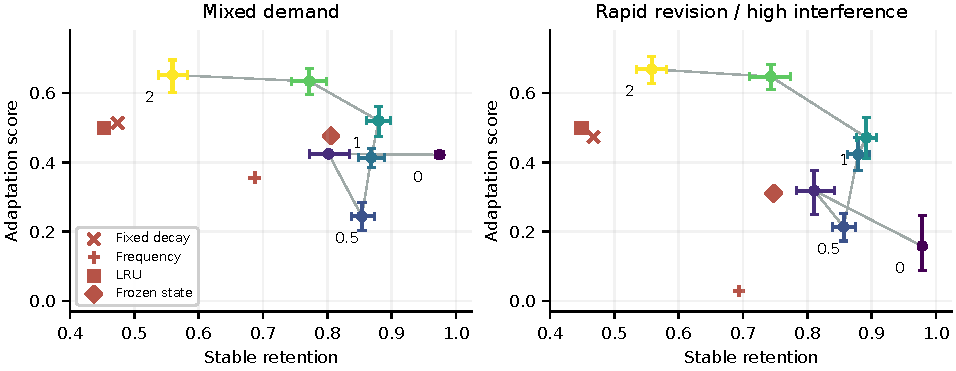
\includegraphics[width=\linewidth]{figures/operating_region.pdf}
\caption{Eight-slot operating points: all seven rates, colored low (purple) to high (yellow), with selected labels and world-level 95\% bootstrap intervals. Lines follow parameter order, not an optimized frontier. All conditions appear in Appendix~\ref{app:operating}.}\label{fig:operating}
\end{figure}
Twenty-seven pairs show opposite endpoint changes with both Holm-adjusted $p<0.05$: nine in mixed demand at capacity 8, twelve in rapid/high at capacity 8, six in rapid/high at capacity 16, and none in mixed demand at capacity 16. These pairs share worlds and parameters; 27 is not a count of independent replications.

In rapid/high capacity 8, moving from $\alpha=1$ to $2$ raises AS from 0.472 to 0.669 ($\Delta=0.197$, CI $[0.141,0.251]$), while SR falls from 89.19\% to 55.82\% ($\Delta=-33.38$ points, CI $[-36.02,-30.67]$); both adjusted $p=0.0168$. This is a direct operating-point trade-off without additional fitting. Some intermediate strengths are dominated, and retention saturates in mixed demand at capacity 16. Static comparators are fixed configurations, not equally extensive hyperparameter families: these experiments establish tunability of \ame, not its uniqueness or superiority to every tunable heuristic.
